\section{Alternative methods of discrete variational inference}

We can gain insight and intuition about the stick-breaking and
rounding transformations by considering their counterparts for
discrete, or categorical, variational inference.  Continuous
relaxations are an appealing approach for this problem, affording
gradient-based inference with the reparameterization trick.
First we review the Gumbel-softmax method~\citep{maddison2016concrete,
  jang2016categorical, kusner2016gans}---a recently proposed
method for discrete variational inference with the reparameterization
trick---then we discuss analogs of our permutation and rounding
transformations for the categorical case.  These can be considered
alternatives to the Gumbel-softmax method, which we compare
empirically in Appendix~\ref{sec:vae}.

Recently there have been a number of proposals for extending the
reparameterization trick~\citep{rezende2014stochastic, Kingma2014} to
high dimensional discrete problems\footnote{Discrete inference is only
  problematic in the high dimensional case, since in low dimensional
  problems we can enumerate the possible values of~$x$ and compute the
  normalizing constant~$p(y) = \sum_x p(y, x)$.} by relaxing them to
analogous continuous problems \citep{maddison2016concrete,
  jang2016categorical, kusner2016gans}.  These approaches are based on
the following observation: if~$x \in \{0,1\}^N$ is a one-hot vector
drawn from a categorical distribution, then the support of~$p(x)$ is
the set of vertices of the~$N-1$ dimensional simplex.  We can
represent the distribution of~$x$ as an atomic density on the simplex.

\subsection{The Gumbel-softmax method}
Viewing~$x$ as a vertex of the simplex motivates a natural relaxation:
rather than restricting ourselves to atomic measures,
consider continuous densities on the simplex. To be concrete, suppose
the density of~$x$ is defined by the transformation,
\begin{align*}
  \noise_n &\iid{\sim} \mathrm{Gumbel}(0, 1) \\
  \psi_n & = \log \theta_n + \noise_n  \\
  x &=  \mathsf{softmax}(\psi / \tau) \\
        &=\left(\frac{e^{\psi_1 / \tau}}{\sum_{n=1}^N e^{\psi_n / \tau}},
      \,\ldots,\,
      \frac{e^{\psi_N / \tau}}{\sum_{n=1}^N e^{\psi_n / \tau}} \right).
\end{align*}
The output~$x$ is now a point on the simplex, and the
parameter~${\theta = (\theta_1, \ldots, \theta_N) \in \reals^N_+}$ can be optimized
via stochastic gradient ascent with the reparameterization trick.

The Gumbel distribution leads to a nicely interpretable model: adding
i.i.d. Gumbel noise to~${\log \theta}$ and taking the argmax yields an
exact sample from the normalized probability mass
function~$\bar{\theta}$,
where~${\bar{\theta}_n = \theta_n / \sum_{m=1}^N
  \theta_m}$~\citep{gumbel1954statistical}. The softmax is a natural
relaxation. As the temperature~$\tau$ goes to zero, the softmax
converges to the argmax function. Ultimately, however, this is just a
continuous relaxation of an atomic density to a continuous density.

Stick-breaking and rounding offer two alternative ways of constructing a
relaxed version of a discrete random variable, and both are amenable
to reparameterization. However, unlike the Gumbel-Softmax, these
relaxations enable extensions to more complex combinatorial objects,
notably, permutations.

\subsection{Stick-breaking}

The stick-breaking transformation to the Birkhoff polytope presented
in the main text contains a recipe for stick-breaking on the simplex.
In particular, as we filled in the first row of the doubly-stochastic
matrix, we were transforming a real-valued vector~$\psi \in \reals^{N-1}$
to a point in the simplex.  We present this procedure for
discrete variational inference again here in simplified form.
Start with a reparameterization of a Gaussian vector,
\begin{align*}
  \noise_n &\iid{\sim} \distNormal(0, 1), \\
  \psi_n & = \mu_n + \nu_n \noise_n, \qquad 1 \leq n \leq N-1,
\end{align*}
parameterized by~${\theta = (\mu_n, \nu_n)_{n=1}^{N-1}}$. 
Then map this to the unit hypercube in a temperature-controlled manner
with the logistic function,
\begin{align*}
  \beta_n &= \sigma(\psi_n / \tau),
\end{align*}
where~${\sigma(u) = (1+e^{-u})^{-1}}$ is the logistic function.
Finally, transform the unit hypercube to a point in the simplex:
\begin{align*}
  x_1 &= \beta_1, \\
  x_n &= \beta_n \left(1- \sum_{m=1}^{n-1} x_m\right), \qquad 2 \leq n \leq N-1,  \\
  x_N &= 1- \sum_{m=1}^{N-1} x_m,
\end{align*}
Here,~$\beta_n$ is the fraction of the remaining ``stick'' of probability
mass assigned to~$x_n$.  This transformation is invertible, the
Jacobian is lower-triangular, and the determinant of the Jacobian is
easy to compute.  \citet{linderman2015dependent} compute the density
of~$x$ implied by a Gaussian density on~$\psi$.

The temperature~$\tau$ controls how concentrated~$p(x)$ is at the
vertices of the simplex, and with appropriate choices of parameters,
in the limit~${\tau \to 0}$ we can recover any categorical
distribution (we will discuss this in detail in
Section~\ref{sec:sblimits}. In the other limit, as~$\tau \to \infty$,
the density concentrates on a point in the interior of the simplex
determined by the parameters, and for intermediate values, the density
is continuous on the simplex.

Finally, note that the logistic-normal construction is only one
possible choice.  We could instead
let~${\beta_n \sim \mathrm{Beta}(\tfrac{a_n}{\tau},
  \tfrac{b_n}{\tau})}$. This would lead to a generalized Dirichlet
distribution on the simplex.  The beta distribution is slightly harder
to reparameterize since it is typically simulated with a rejection
sampling procedure, but~\citet{naesseth2017reparameterization} have
shown how this can be handled with a mix of reparameterization and
score-function gradients.  Alternatively, the beta distribution could
be replaced with the Kumaraswamy
distribution~\citep{kumaraswamy1980generalized}, which is quite
similar to the beta distribution but is easily reparameterizable.

\subsection{Rounding}
Rounding transformations also have a natural analog for discrete
variational inference.  Let~$e_n$ denote a one-hot vector with~$n$-th
entry equal to one.  Define the rounding operator,
\begin{align*}
  \mathsf{round}(\psi)
  &= e_{n^*},
\end{align*}
where
\begin{align*}
  n^* &= \argmin_{n} \|e_n - \psi \|^2 \\
  % &= \argmin_{n} \sum_{m \neq n} \psi_m^2 + (1 - \psi_n)^2  \\
  % &= \argmin_{n} \sum_{m \neq n} \psi_m^2 + \psi_n^2 - 2\psi_n + 1 \\
  % &= \argmin_{n} \|\psi\|^2 - 2\psi_n + 1 \\
  &= \argmax_n \psi_n.
\end{align*}
In the case of a tie, let~$n^*$ be the smallest index~$n$ such
that~$\psi_n > \psi_m$ for all~$m < n$. Rounding effectively
partitions the space into~$N$ disjoint ``Voronoi'' cells,
\begin{align*}
  V_n &= \Big \{ \psi \in \reals^N : \,
        \psi_n \geq \psi_m \, \forall m \; \wedge \;
        \psi_n > \psi_m \, \forall m < n
        \Big \}.
\end{align*}
By definition,~${\mathsf{round}(\psi) = e_{n^*}}$ for
all~${\psi \in V_{n^*}}$


We define a map that pulls points toward their rounded values,
\begin{align}
  \label{eq:round}
  x &=  \tau \psi + (1-\tau) \mathsf{round}(\psi).
\end{align}

\begin{proposition}
  \label{prop:round}
  For~${\tau \in [0,1]}$, the map defined by~\eqref{eq:round} moves
  points strictly closer to their rounded values so
  that~$\mathsf{round}(\psi) = \mathsf{round}(x)$.
\end{proposition}

\begin{proof}
Note that the Voronoi cells are intersections of halfspaces and, as
such, are convex sets.  Since~$x$ is a convex combination of~$\psi$
and~$e_{n^*}$, both of which belong to the convex set~$V_{n^*}$,
$x$~must belong to~$V_{n^*}$ as well.
\end{proof}

Similarly,~$x$ will be a point on the simplex if an only if~$\psi$ is
on the simplex as well.  By analogy to the rounding transformations
for permutation inference, in categorical inference we use a Gaussian
distribution~${\psi \sim \distNormal(\mathsf{proj}(m), \nu)}$,
where~$\mathsf{proj}(m)$ is the projection of~$m \in \reals_+^N$ onto
the simplex.  Still, the simplex has zero measure under the Gaussian
distribution.  It follows that the rounded points~$x$ will almost
surely not be on the simplex either.  The supposition of this approach
is that this is not a problem: relaxing to the simplex is nice but not
required.

In the zero-temperature limit we obtain a discrete distribution on the
vertices of the simplex.  For~${\tau \in (0,1]}$ we have a
distribution on~${\mcX_\tau \subseteq \reals^N}$, the subset of the
reals to which the rounding operation maps. (For~${0 \leq \tau < 1}$
this is a strict subset of~$\reals^N$.) To derive the
density~$q(x)$, we need the inverse transformation and the
determinant of its Jacobian.  From Proposition~\ref{prop:round}, it
follows that the inverse transformation is given by,
\begin{align*}
  \psi &= \frac{1}{\tau} x - \frac{1 - \tau}{\tau} \mathsf{round}(x).
\end{align*}
As long as~$\psi$ is in the interior of its Voronoi cell,
the~$\mathsf{round}$ function is piecewise constant and the
Jacobian is~${\tfrac{\partial\psi}{\partial x} = \tfrac{1}{\tau} I}$,
and its determinant is~$\tau^{-N}$. Taken together, we have,
\begin{multline*}
  q(x; m, \nu) =  \\
  \tau^{-N} \distNormal \left(\frac{1}{\tau}x - \frac{1-\tau}{\tau} \mathsf{round}(x); \, \mathsf{proj}(m), \diag(\nu) \right) \\
  \times \bbI[x \in \mcX_\tau].
\end{multline*}
Compare this to the density of the rounded random variables for
permutation inference. 

\subsection{Limit analysis for stick-breaking}
\label{sec:sblimits}
We show that stick-breaking for discrete variational inference can
converge to any categorical distribution in the zero-temperature
limit.
% To do so, we first show that
% in the zero-temperature limit, the distribution
% of~${\sigma(\psi_n / \tau)}$ converges to a Bernoulli distribution.
% The we show that when~$\sigma(\psi_n / \tau)$ is Bernoulli (rather
% than a continuous density on the unit interval), the distribution
% on~$x$ obtained by applying the stick-breaking transformation
% to~$\psi$ is categorical.

% \begin{proposition}
%   \label{prop:bernoulli}
  Let~${\beta=\sigma(\psi / \tau)}$
  with~${\psi\sim\mathcal{N}(\mu,\nu^2)}$.  In the
  limit~${\tau \to
    0}$ we have~${\beta \sim \distBernoulli(\Phi(-\tfrac{\mu}{\nu}))}$,
  where~$\Phi(\cdot)$ denotes the Gaussian cumulative distribution
  function (cdf). 
% \end{proposition}
  % \begin{proof}
  % To see this, let~$F_\beta$ be the cdf of the random
  % variable~$\beta$. Since~$\beta$ is a random variable on the unit interval,
  % $F_\beta$ is a non-decreasing function on~$[0,1]$ with~${F_\beta(0)=0}$
  % and~${F_\beta(1)=1}$.  Reparameterize~${\psi = \mu + \nu \noise}$
  % where~${\noise \sim \distNormal(0,1)}$. Then we have,
  % \begin{align*}
  %   F_\beta(u) &= \Pr(\sigma(\psi / \tau) < u) \\
  %        &= \Pr(\psi < \tau \sigma^{-1}(u)) \\
  %        &= \Pr(\noise < \tfrac{\tau}{\nu} \sigma^{-1}(u) - \tfrac{\mu}{\nu}))\\
  %        &= \Phi(-\tfrac{\tau}{\nu}\sigma^{-1}(u) - \tfrac{\mu}{\nu}).
  % \end{align*}
  % By the continuity of~$\Phi$ we have,
  % \begin{align*}
  %   \lim_{\tau \to 0} F_\beta(u) &= \Phi(-\tfrac{\mu}{\nu}) &
  %   \text{for } u &\in (0,1).
  % \end{align*}
  % This is the cdf of a Bernoulli random with
  % probability~${\rho = \Phi(-\tfrac{\mu}{\nu})}$.
  % \end{proof}
  %
% \begin{proposition}
%   \label{prop:categorical}
%   As above, let~${\beta_n=\sigma(\psi_n / \tau)}$.
  Moreover, when~${\beta_n \sim \distBernoulli(\rho_n)}$
  with~${\rho_n \in [0,1]}$ for~${n=1, \ldots, N}$, the random
  variable~$x$ obtained from applying the stick-breaking
  transformation to~$\beta$ will have an atomic distribution with atoms
  in the vertices of $\Delta_{N}$; i.e,
  ${x \sim \distCategorical(\pi)}$ where
  \begin{align*}
    \pi_1 &= \rho_1 \\
    \pi_n &=  \rho_n \prod_{m=1}^{n-1} (1-\rho_m)  \qquad
          n=2, \ldots, N-1, \\
    \pi_N &= \prod_{m=1}^{N-1} (1-\rho_m).
\end{align*}
% \end{proposition}

% \begin{proof}
%   From the stick-breaking definition,~${x_1 = \beta_1}$,
%   ${x_n = \beta_n (1- \sum_{m < n} x_m)}$,
%   and~${x_N = 1-\sum_{m < N} x_m}$.
%   When~${\beta_n \in \{0,1\}}$ for all~${n = 1, \ldots, N-1}$,
%   we have the following equivalencies. For the first element,
%   \begin{align*}
%     x_1 = 1 &\iff \beta_1 = 1;
%   \end{align*}
%   for~${1 < n < N-1}:$
%   \begin{align*}
%     x_n = 1 &\iff (\beta_n = 1) \bigwedge_{m=1}^{n-1} (\beta_m = 0);
%   \end{align*}
%   and for the last element,
%   \begin{align*}
%     x_N = 1 &\iff \bigwedge_{m=1}^{N-1} (\beta_m = 0).
%   \end{align*}
%   These events are mutually exclusive, implying that~$x$ will
%   necessarily be a one-hot vector, i.e. a categorical random variable.
%   Since~$\beta_1, \ldots, \beta_{N-1}$ are independent Bernoulli random
%   variables, the probabilities of these events are given
%   by the~${\pi, \ldots, \pi_N}$ stated in the proposition. 
% \end{proof}

These two facts, combined with the invertibility of the
stick-breaking procedure, lead to the following proposition

\begin{proposition}
  In the zero-temperature limit, stick-breaking of logistic-normal
  random variables can realize any categorical distribution on~$x$.
\end{proposition}

\begin{proof}
  There is a one-to-one correspondence between~${\pi \in \Delta_N}$
  and~${\rho \in [0,1]^{N-1}}$.  Specifically,
  \begin{align*}
    \rho_1 &= \pi_1 \\
    \rho_n &= \frac{\pi_n}{\prod_{m=1}^{n=1} 1-\rho_m}
             \quad \text{for } n = 2, \ldots, N-1.
  \end{align*}
  Since these are recursively defined, we can substitute the
  definition of~$\rho_m$ to obtain an expression for~$\rho_n$ in terms
  of~$\pi$ only.  Thus, any desired categorical distribution~$\pi$
  implies a set of Bernoulli parameters~$\rho$.  In the zero
  temperature limit, any desired~$\rho_n$ can be obtained with
  appropriate choice of Gaussian mean~$\mu_n$ and
  variance~$\nu_n^2$. Together these imply that stick-breaking can
  realize any categorical distribution when~${\tau \to 0}$.
\end{proof}


\subsection{Variational Autoencoders (VAE) with categorical latent variables}
\label{sec:vae}


We considered the density estimation task on MNIST digits, as in
\citet{maddison2016concrete, jang2016categorical}, where observed
digits are reconstructed from a latent discrete code. We used the
continuous ELBO for training, and evaluated performance based on the
marginal likelihood, estimated with the variational
objective of the discretized model.  We compared against the methods of
\cite{jang2016categorical, maddison2016concrete} and obtained the
results in Table~\ref{tab:vae}.  While stick-breaking and rounding
fare slightly worse than the Gumbel-softmax method, they are readily
extensible to more complex discrete objects, as shown in the main
paper.

\begin{table}[h]
  \caption{Summary of results in VAE}
  \label{tab:vae}
  \centering
  \begin{tabular}{ll}
    \textbf{Method} & $- \log p(x)$ \\
    \hline
    Gumbel-Softmax    & 106.7 \\
    Concrete  &  111.5\\
    Rounding &  121.1 \\
    Stick-breaking & 119. 8\\
    \bottomrule
  \end{tabular}
\end{table}


% \begin{table*}[t]
%   \caption{Battacharya distances in the synthetic matching experiment}
%   \label{sample-table}
%   \centering
%   \begin{tabular}{llllllll}
%    & \multicolumn{1}{c}{Rounding} & \multicolumn{1}{c}{Stick-breaking} & \multicolumn{5}{c}{Mallows}\\
%     \cmidrule(lr){2-2} \cmidrule(lr){3-3} \cmidrule(lr){4-8}
%     &    & &   $\theta=0.1$ &  $\theta=1$ & $\theta=2$ & $\theta=5$ & $\theta=10$ \\
%     \midrule
%     $\sigma=0.1$     & .06 & .09  &.93 &.51& .23  & .08 &.08\\
%     $\sigma=0.25$     & .21 & .23 & .92 &.53 & .33&  .27 &.27\\
%      $\sigma=0.5$     & .32 & .41 & .89 &.61 & .53&  .54& .54\\
%      $\sigma=0.75$     & .38   & .55 & .85 &.71 & .69&  .72 &.72\\
   
%     \bottomrule
%   \end{tabular}
% \end{table*}

Figure~\ref{fig:VAE} shows MNIST reconstructions using Gumbel-Softmax,
stick-breaking and rounding reparameterizations. In all the three
cases reconstructions are reasonably accurate, and there is diversity
in reconstructions.
\begin{figure*}[t]
  \centering
  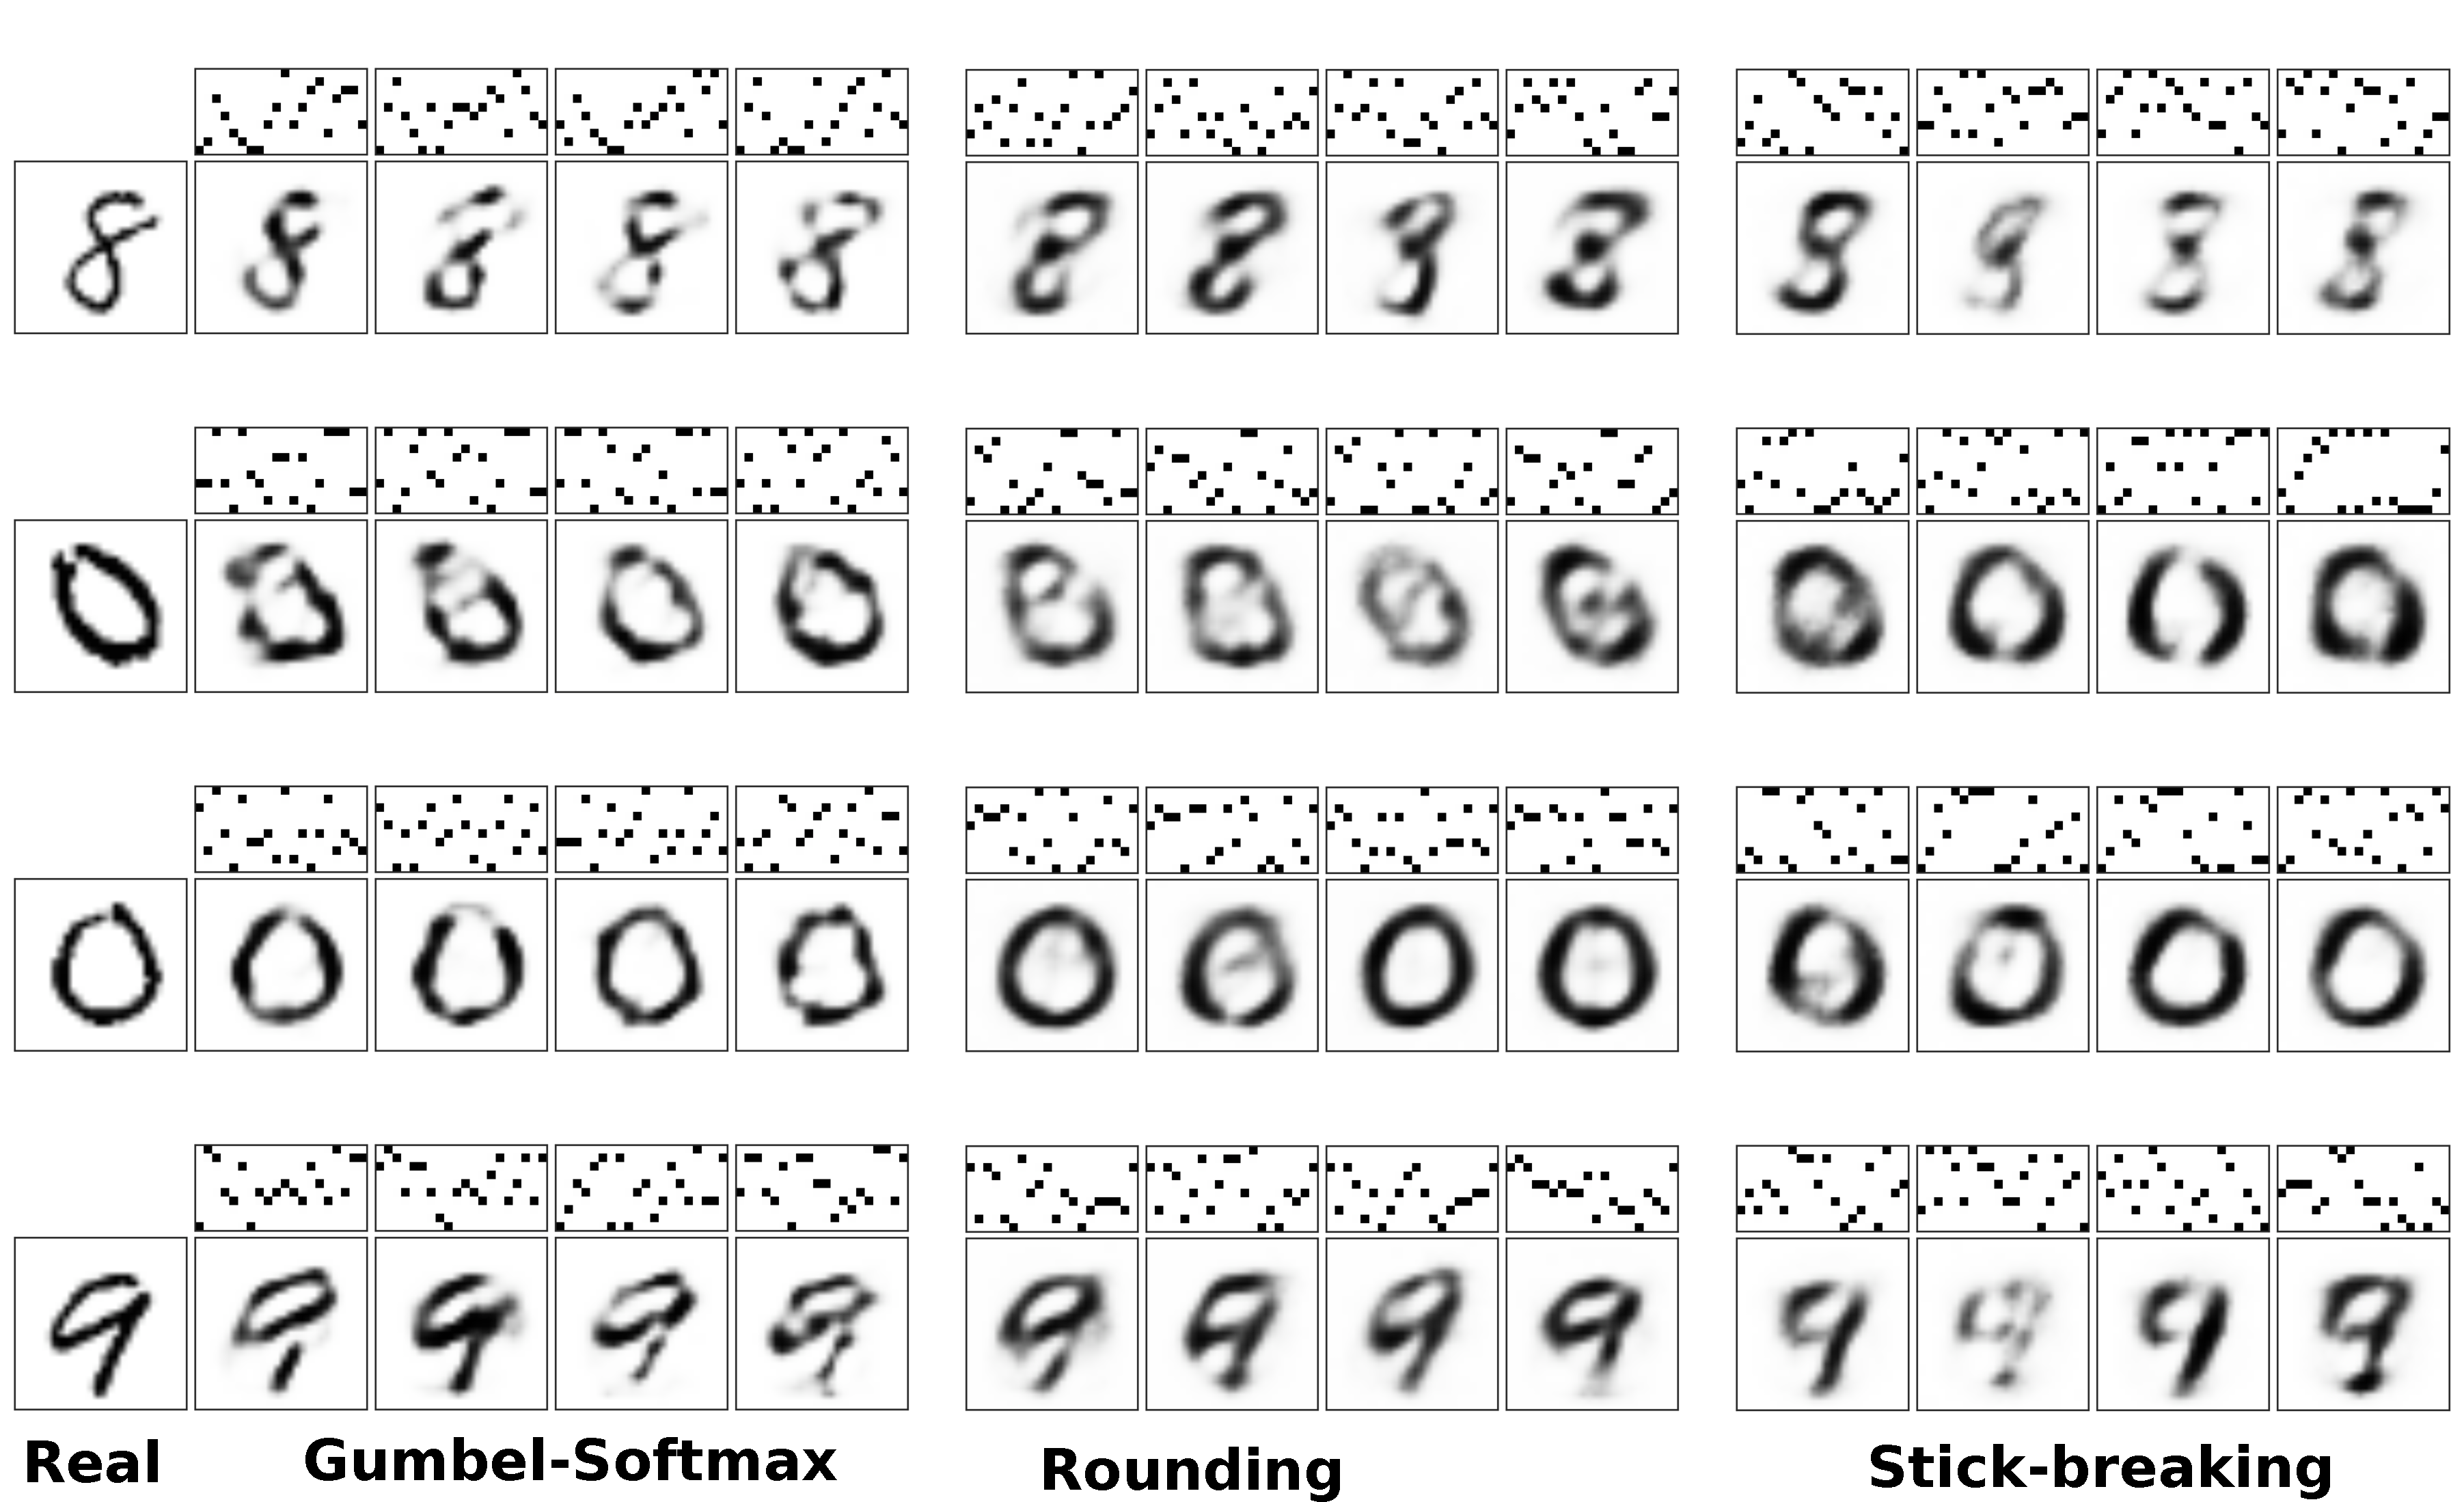
\includegraphics[width=5.in]{figure4.pdf} 
  \caption{\textit{Examples of true and reconstructed digits from their
    corresponding discrete latent variables.} The real input image is
    shown on the left, and we show sets of four samples from the
    posterior predictive distribution for each discrete variational
    method: Gumbel-softmax, rounding, and stick-breaking.  Above each
    sample we show the corresponding sample of the discrete latent
    ``code.''  The random codes consist of of~$K=20$ categorical
    variables with $N=10$ possible values each.  The codes are shown
    as~${10 \times 20}$~binary matrices above each image.}
\label{fig:VAE}
\end{figure*}


\section{Variational permutation inference details}
\label{sec:details}

Here we discuss more of the subtleties of variational permutation
inference and present the mathematical derivations in more detail. 

\subsection{Continuous prior distributions.} 
Continuous relaxations require re-thinking the objective: the model
log-probability is defined with discrete latent variables, but our
relaxed posterior is a continuous density. As in
\cite{maddison2016concrete}, we instead maximize a relaxed ELBO.  We
assume the functional form of the likelihood remains unchanged, and
simply accepts continuous values instead of discrete. However, we need
to specify a new continuous prior $p(X)$ over the relaxed discrete
latent variables, here, over relaxations of permutation matrices. It
is important that the prior be sensible: ideally, the prior should
penalize values of~$X$ that are far from permutation matrices.

For our categorical experiment on MNIST we use a mixture of Gaussians
around each
vertex,~${p(x) = \tfrac{1}{N} \sum_{n=1}^N \mathcal{N}(x \given e_k,
  \eta^2)}$.  This can be extended to permutations, where we use a
mixture of Gaussians for each coordinate,
\begin{align}
\label{eq:permprior}
  p(X) &= \prod_{m=1}^N \prod_{n=1}^N
  \frac{1}{2} \left(\mathcal{N}(x_{mn} \given 0, \eta^2) + \distNormal(x_{mn} \given 1, \eta^2 \right).
\end{align}
Although this prior puts significant mass around invalid points
(e.g.~${(1, 1, \ldots, 1)}$), it penalizes~$X$ that are far from~$\mcB_N$.

\subsection{Computing the ELBO}
Here we show how to evaluate the ELBO.  Note that the stick-breaking
and rounding transformations are compositions of invertible
functions,~${g_\tau = h_\tau \circ f}$ with ${\Psi = f(\noise; \theta)}$ and
${X = h_\tau(\Psi)}$.  In both cases,~$f$ takes in a matrix of
independent standard Gaussians~$(\noise)$ and transforms it with the
means and variances in~$\theta$ to output a matrix~$\Psi$ with
entries~${\psi_{mn} \sim \distNormal(\mu_{mn}, \nu^2_{mn})}$.
Stick-breaking and rounding differ in the temperature-controlled
transformations~$h_\tau(\Psi)$ they use to map~$\Psi$ toward the
Birkhoff polytope.

To evaluate the ELBO, we must compute the density
of~$q_\tau(X; \theta)$.
Let~${J_{h_\tau}(u) = \frac{\partial h_\tau(U)}{\partial U}
  \big|_{U=u}}$ denote the Jacobian of a function~$h_\tau$ evaluated
at value~$u$. By the change of variables theorem and properties of the
determinant,
\begin{align*}
  q_\tau(X; \theta)
  &= p \big(h_\tau^{-1}(X) ;\theta \big)
    \times \big| J_{h_\tau^{-1}}(X) \big|
  \\
  &= p \big(h_\tau^{-1}(X); \theta \big)
    \times \big| J_{h_\tau}(h_\tau^{-1}(X)) \big|^{-1}.
\end{align*}
Now we appeal to the law of the unconscious statistician to compute
the entropy of~$q_\tau(X; \theta)$,
\begin{align}
  \label{eq:elbo2}
  \nonumber \E_{q_\tau(X; \theta)} & \Big[- \log q(X; \theta) \Big] \\
  \nonumber &= \E_{p(\Psi;\theta)}
              \Big[ - \log p(\Psi;\theta) +
              \log \left| J_{h_\tau}(\Psi) \right| \Big] \\
  &= \bbH(\Psi; \theta)  +
  \E_{p(\Psi;\theta)} \Big[ \left| J_{h_\tau}(\Psi) \right| \Big].
\end{align}
Since~$\Psi$ consists of independent Gaussians with
variances~$\nu_{mn}^2$, the entropy is simply,
\begin{align*}
  \bbH(\Psi; \theta) &=  \frac{1}{2} \sum_{m,n} \log(2 \pi e \nu_{mn}^2).
\end{align*}
We estimate the second term of equation \eqref{eq:elbo2} using
Monte-Carlo samples. For both transformations, the Jacobian has a
simple form.

\paragraph{Jacobian of the stick-breaking transformation.}
Here~$h_\tau$ consists of two steps:
map~${\Psi \in \reals^{N-1 \times N-1}}$
to~$B \in [0,1]^{N-1 \times N-1}$ with a temperature-controlled,
elementwise logistic function, then map~$B$ to~$X$ in the Birkhoff
polytope with the stick-breaking transformation.

As with the standard stick-breaking transformation to the simplex,
our transformation to the Birkhoff polytope is feed-forward;
i.e. to compute~$x_{mn}$ we only need to know the values of~$\beta$
up to and including the~$(m,n)$-th entry. Consequently, the
Jacobian of the transformation is triangular, and its determinant
is simply the product of its diagonal.

We derive an explicit form in two steps. With a slight abuse of
notation, note that the Jacobian of~$h_\tau(\Psi)$ is given
by the chain rule,
\begin{align*}
  J_{h_\tau}(\Psi)
  &= \frac{\partial X}{\partial  \Psi}
    = \frac{\partial X}{\partial B} \frac{\partial B}{\partial \Psi}.
\end{align*}
Since both transformations are bijective, the determinant is,
\begin{align*}
  \big| J_{h_\tau}(\Psi) \big|
  &= \left| \frac{\partial X}{\partial B} \right| \,
     \left| \frac{\partial B}{\partial \Psi} \right|.
\end{align*}
the product
of the individual determinants.  The first determinant is,
\begin{align*}
  \left| \frac{\partial X}{\partial B} \right|
  &= \prod_{m=1}^{N-1} \prod_{n=1}^{N-1} \frac{\partial x_{mn} }{\partial {\beta}_{mn}} 
  = \prod_{m=1}^{N-1} \prod_{n=1}^{N-1} (u_{mn} - \ell_{mn}).
\end{align*}
The second transformation, from~$\Psi$ to~$B$, is an element-wise,
temperature-controlled logistic transformation such that,
\begin{align*}
  \left| \frac{\partial B}{\partial \Psi} \right| 
  &= \prod_{m=1}^{N-1} \prod_{n=1}^{N-1} \frac{\partial \beta_{mn}}{\partial \psi_{mn}} \\
  &= \prod_{m=1}^{N-1} \prod_{n=1}^{N-1}
    \frac{1}{\tau} \sigma \left(\psi_{mn} / \tau \right)
    \sigma \left(-\psi_{mn} / \tau \right).
\end{align*}

% \begin{align*}
%   &= \prod_{i=1}^{N-1} \prod_{j=1}^{N-1} \frac{\partial}{\partial {x}_{ij}}
%     \sigma^{-1} \left( \frac{{x}_{ij} - \ell_{ij}}{u_{ij} - \ell_{ij}} \right ) \\
%   &= \prod_{i=1}^{N-1} \prod_{j=1}^{N-1}
%     \left( \frac{1}{u_{ij} - \ell_{ij}} \right )
%     \left( \frac{u_{ij} - \ell_{ij}}{{x}_{ij} - \ell_{ij}} \right )
%     \left( \frac{u_{ij} - \ell_{ij}}{u_{ij} - {x}_{ij}} \right ) \\
%   &= \prod_{i=1}^{N-1} \prod_{j=1}^{N-1}
%     \frac{u_{ij} - \ell_{ij}}{({x}_{ij} - \ell_{ij}) (u_{ij} - {x}_{ij})}
% \end{align*}

% To compute the gradient of the forward transformation $h$, one simply needs to invert the above (or put a negative sign, in the logarithm scale). Finally,  to incorporate the effect of $\sigma$ ($B=\sigma(\Psi)$), by the chain rule,  one only needs to add a term corresponding to this derivative, $d\sigma(x)/dx=\sigma(x)\sigma(-x)$. 


It is important to note that the transformation that maps
$B \rightarrow X$ is only piecewise continuous: the function is not
differentiable at the points where the bounds change; for example,
when changing~$B$ causes the active upper bound to switch from the row
to the column constraint or vice versa.  In practice, we find
that our stochastic optimization algorithms still perform reasonably
in the face of this discontinuity.


\paragraph{Jacobian of the rounding transformation.}
The rounding transformation is given in matrix form
in the main text, and we restate it here in coordinate-wise form
for convenience,
\begin{align*}
  x_{mn} = [h_\tau(\Psi)]_{mn} &= \tau \psi_{mn} + (1-\tau) [\mathsf{round}(\Psi)]_{mn}.
\end{align*}
This transformation is piecewise linear with jumps at the boundaries
of the ``Voronoi cells;'' i.e., the points where~$\mathsf{round}(X)$
changes. The set of discontinuities has Lebesgue measure zero so the
change of variables theorem still applies.  Within each Voronoi cell,
the rounding operation is constant, and the Jacobian is,
\begin{align*}
  \log \big| J_{h_\tau}(\Psi) \big| = \sum_{m,n} \log \tau = N^2 \log \tau.
\end{align*}
For the rounding transformation with given temperature, the Jacobian
is constant.




\section{Experiment details}
We used Tensorflow \citep{Abadi2016} for the VAE experiments, slightly
changing the code made available from \cite{jang2016categorical}. For
experiments on synthetic matching and the C. elegans example we used
Autograd \citep{maclaurin2015autograd}, explicitly avoiding
propagating gradients through the non-differentiable~$\mathsf{round}$
operation, which requires solving a matching problem.

We used ADAM~\citep{kingma2014adam} with learning rate 0.1 for
optimization. For rounding, the parameter vector $V$ defined in
\ref{sub:rounding} was constrained to lie in the interval
$[0.1, 0.5]$. Also, for rounding, we used ten iterations of the
Sinkhorn-Knopp algorithm, to obtain points in the Birkhoff
polytope. For stick-breaking the variances $\nu$ defined in
\ref{sub:stickbreaking} were constrained between $10^{-8}$ and~$1$. In
either case, the temperature, along with maximum values for the noise
variances were calibrated using a grid search.
 
In the C. elegans example we considered the symmetrized version of the
adjacency matrix described in \citep{varshney2011structural}; i.e. we
used $A'=(A+A^\top)/2$, and the matrix $W$ was chosen antisymmetric,
with entries sampled randomly with the sparsity pattern dictated by
$A'$. To avoid divergence, the matrix $W$ was then re-scaled by 1.1
times its spectral radius. This choice, although not essential,
induced a reasonably well-behaved linear dynamical system, rich in
non-damped oscillations. We used a time window of $T=1000$ time
samples, and added spherical standard noise at each time. All results
in Figure \ref{fig:elegantresults} are averages over five experiment
simulations with different sampled matrices $W$. For results in Figure
\ref{fig:elegantresults}b we considered either one or four worms
(squares and circles, respectively), and for the x-axis we used the values
$\nu \in \{0.0075,0.01,0.02,0.04,0.05\}$. We fixed the number of known neuron
identities to 25 (randomly chosen). For results in Figure
\ref{fig:elegantresults}c we used four worms and considered two values
for $\nu$; 0.1 (squares) and 0.05 (circles). Different x-axis values
correspond to fixing 110, 83, 55 and 25 neuron identities.
